\subsection{Estándares EN-50126, EN-50128 y EN-50129}
	\label{sec:normas}
	
    El estándar internacional IEC 61508 \cite{Paper_77,Paper_78,Paper_79,Paper_80,Paper_81,Paper_82,Paper_83} es la base para definir un conjunto de estrategias y buenas prácticas para ser aplicadas en el diseño de sistemas críticos, eléctricos y electrónicos, en diversas industrias \cite{Paper_26,Paper_29,Paper_30,Paper_31,Paper_34,Paper_47}. Entre las industrias alcanzadas por los lineamientos básicos establecidos en la IEC 61508 se encuentran la industria nuclear, la industria automotriz y la industria ferroviaria, como se puede visualizar en la Figura \ref{fig:IEC_61508}.

    \begin{figure}[H]
        \centering
        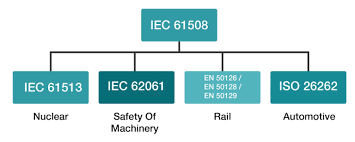
\includegraphics[width=1\textwidth]{Figuras/IEC61508.png}
        \centering\caption{Estándar IEC 61508.}
        \label{fig:IEC_61508}
    \end{figure}

    Dentro del universo de estándares ferroviarias, nos enfocaremos principalmente en tres de ellas: EN-50126 \cite{Paper_70,Paper_71,Paper_72,Paper_73,Paper_74}, EN-50128 \cite{Paper_75,Paper_74} y EN-50129 \cite{Paper_76,Paper_73}. Una falla en un sistema crítico puede poner en peligro cientos de vidas humanas y/o dañar la costosa infraestructura del sistema. Es por eso que los sistemas de enclavamiento deben cumplir los estrictos parámetros de fiabilidad, disponibilidad, mantenibilidad y seguridad (RAMS, del inglés Reliability, Availability, Mantenibility and Safety), durante todo el ciclo de vida definido en el estándar EN-50126 \cite{Paper_70,Paper_66,Paper_84}.

    Adicionalmente, el estándar EN-50126 define el nivel de integridad de seguridad (SIL, del inglés Safety Integrity Level). Este parámetro no es del sistema en su conjunto, sino que se asocia a las funciones de seguridad asociadas al sistema, pudiendo tener diferentes SILs dentro de un mismo dispositivo. Se definen cuatro niveles SIls, siendo el cuatro el nivel mas alto y, por lo tanto, el que tiene una tasa de fallas menor. Aunque existen diversos factores que impactan en la determinación del SIL, podemos tomar como referencia el criterio definido en la Tabla \ref{Tab:tabla_SIL} en función de la probabilidad de fallas por hora (PFH) del sistema funcionando de forma continua.

    \begin{table}[H]
        {
        \caption{SIL en función de la Probabilidad de Fallas/Hora (PFH).}
        \label{Tab:tabla_SIL}
        \centering
        %\small
            %\centering
            \begin{center}
            \resizebox{0.75\textwidth}{!}{
            \begin{tabular}{ c | c c c c c }
                %\hline	
                   SIL & & & & &  \\	
                \hline
                   4 & $10^{-8}$ & \multirow{4}{*}{$>$} & \multirow{4}{*}{PFH} & \multirow{4}{*}{$>$} & $10^{-9}$ \\
                   3 & $10^{-7}$ & &  & & $10^{-8}$ \\
                   2 & $10^{-6}$ & &  & & $10^{-7}$ \\
                   1 & $10^{-5}$ & &  & & $10^{-6}$ \\
                %\hline
            \end{tabular}
            }
            \end{center}
        }    
    \end{table}

    El estándar EN-50128 establece las buenas prácticas, metodologías y técnicas aplicables en el área de software para lograr el SIL objetivo. Algunas de estas técnicas pueden ser obligatorias, altamente recomendadas, recomendadas, desaconsejadas o prohibidas \cite{Paper_75,Paper_15,Paper_21,Paper_40,Paper_48,Paper_50,Paper_54,Paper_65}. En algunos casos es obligatorio elegir entre diferentes combinaciones de metodologías optativas. Podemos encontrar entre estas: evitar el uso de punteros, elegir un lenguaje fuertemente tipado, modularizar el código, prohibición de usar memoria dinámica, entre otras \cite{Paper_27,Paper_33,Paper_39,Paper_75}. Este estándar solo se aplica si el sistema incluye un microprocesador con software embebido.

    El estándar EN-50129 es el equivalente en hardware al estándar EN-50128. Las metodologías definidas en EN-50129 se centran en la elección de componentes electrónicos \cite{Paper_68,Paper_116,Paper_117,Paper_120,Paper_122,Paper_126}, compatibilidad electromagnética y dos conceptos fundamentales: redundancia \cite{Paper_23,Paper_29,Paper_32,Paper_42,Paper_49,Paper_97,Paper_98} y diversidad \cite{Paper_53,Paper_125,Paper_131,Paper_132,Paper_140,Paper_171}.

    